\chapter{A Theoretical Comparison of the Effect of Bicycle Lean on the Travel Path of the Bicycle}
\label{Chap:A}
\pagestyle{headings}

\section{Introduction}
Bicycles don't travel along a perfectly straight line. Even when in a seated posture riders make regular small adjustments to keep the system's CoM above the BoS. When shifting to a non-seated posture these adjustments become much larger but less frequent. The lean angle of the bicycle will cause the path of the bicycle to arc away from the imaginary straight line connecting the point from which you start to where you finish. The magnitude and frequency of these deviations may combine to impact performance depending on whether resistance to forward motion is due to conservative forces (i.e. gaining potential energy) or non-conservative forces (i.e. air resistance). We can see in Figure \ref{fig:travelpath} that the smooth periodic oscillations resemble that of a sine wave.
    
\begin{figure}[htbp]
    \centering
    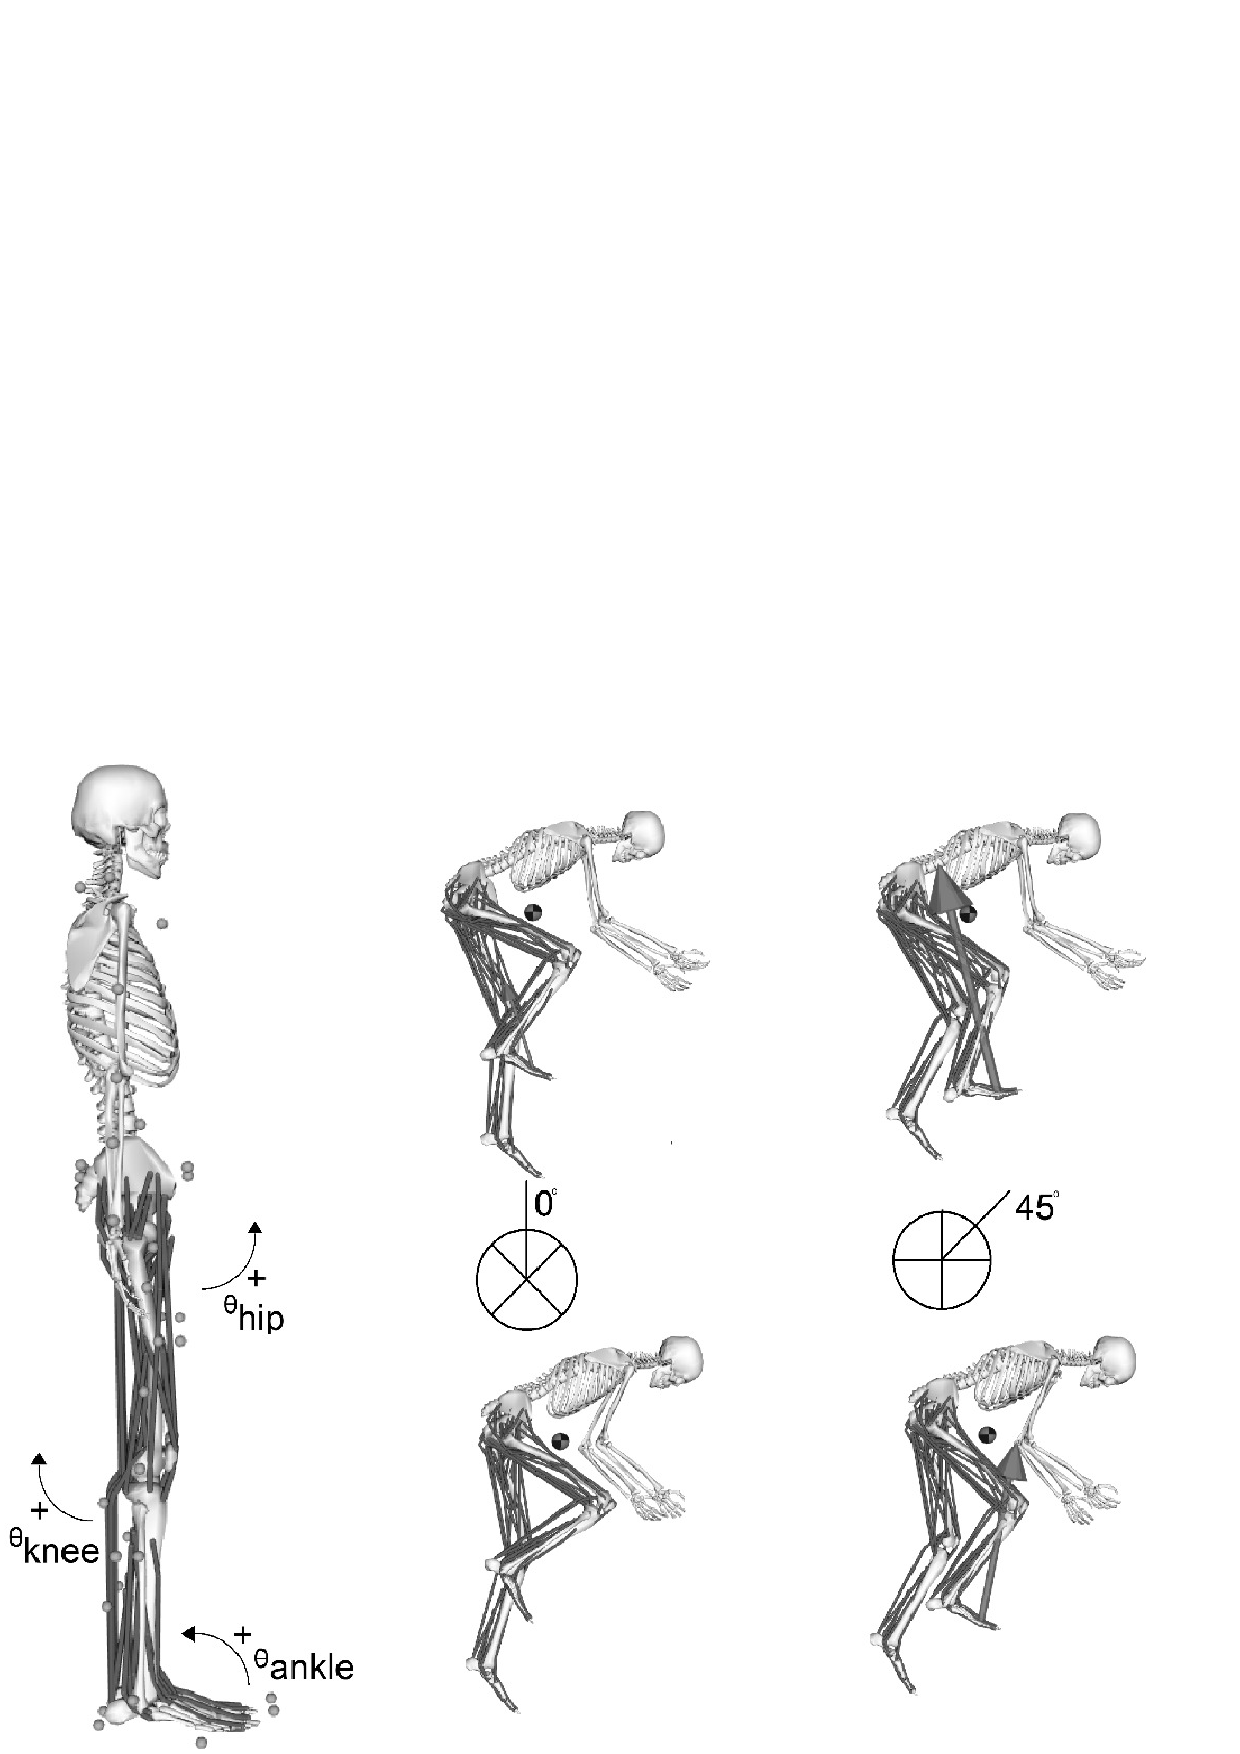
\includegraphics[width=\textwidth]{Study4/Figure1.png}
    \caption[Leaning and steer of the bicycle increases the path length between two points.]{\textbf{Leaning and steer of the bicycle increases the path length between two points.} Shown here is an aerial view of the theoretical travel path of a bicycle due to lean and steer compared to a straight path. In reality the front and rear wheels do not take the same path, therefore this example would perhaps be more representative of the path taken by the bicycle's CoM. \textit{Data calculated using Equation \ref{eq:angle} and the hypothetical level sprinting scenario outlined in Table \ref{tab:pathlength}.}}
    \label{fig:travelpath}
\end{figure}

One argument against using bicycle lean is that it may increase the path length that a rider must travel between two points. Let's use an example of two common scenarios where riders use a non-seated posture to examine the possible effect of this increase in path length (See Table \ref{tab:pathlength}). 

\section{Theoretical evaluation of path length}
Our two scenarios are a 250 m low-velocity uphill climb and a 250 m high-velocity level sprint for the finish line. We will assume in both scenarios that the amplitude (A) of the sine wave is 0.25 m (See Figure \ref{fig:travelpath}). This means the peak perpendicular distance the bicycle deviates away from the straight path in either direction is $\pm$ 0.25 m. To calculate the wave length ($\lambda$) we need to know the circumference of the bicycle tyre and the gain ratio of the drive train. The typical tyre size used in road racing is known as a ``700x23C'', which has a circumference of 2.096 m. The gain ratio of the drive train is calculated by dividing the number of teeth on the front chain ring by the number of teeth on the rear sprocket connected by the chain. If cadence is known we can calculate the velocity of the bicycle by dividing the wave length by the time taken to complete one crank revolution. The time taken to complete one crank revolution can be calculated by dividing the number of seconds per minute by the number of crank revolutions per minute. Next we use the amplitude (A) and wave length ($\lambda$) to create our function with respect to the distance travelled (Equation \ref{eq:angle}). Once we have our function we can then use numerical integration to find the length of a curve using the arc length formula (Equation \ref{eq:arc}). 

\begin{equation}
    f(x) = A \cdot sin(\frac{2\pi}{\lambda}\cdot x) + d
\label{eq:angle}
\end{equation}

\begin{equation}
    L = \int_{a}^{b}\sqrt{1+[f'(x)]^2 dx}
    \label{eq:arc}
\end{equation}

Finally, we can use the results of our integration to speculate about the impact of this increase in path length on many outcomes such as the increase in time taken to travel a set distance. The increase in time is simply calculated by dividing the increase in path length (250$-$L) by velocity.

\begin{table}[htbp]
    \centering
    \begin{tabular}{l|c|c}
        & \multicolumn{2}{c}{\textbf{Scenario}} \\
        & \textbf{Uphill climb} & \textbf{Level sprint} \\
        \hline
        Straight line distance (m) & 250 & 250 \\
        Wheel circumference (m) & 2.096 & 2.096 \\
        Number of teeth on front chain ring & 39 & 53 \\
        Number of teeth on rear sprocket & 25 & 11 \\
        Pedalling cadence (rpm) & 70 & 120 \\
        Amplitude of deviations (m) & 0.25 & 0.25 \\
        \\
        & \multicolumn{2}{c}{\textbf{Result}} \\
        & \textbf{Uphill climb} & \textbf{Level sprint} \\
        \hline
        Total path length (m) & 263.86 & 251.51 \\
        Increase in path length (m) & 13.86 & 1.51 \\
        Relative increase in path length ($\%$) & 5.54 & 0.60 \\
        Velocity (m$\cdot$s$^{-1}$) & 3.81 & 20.20 \\
        Time taken to travel new path length (s) & 69.17 & 12.45 \\
        Increase in time versus straight line (s) & 3.63 & 0.075 \\ 
    \end{tabular}
    \caption[Leaning the bicycle at low velocity increases path length more so than at high velocity.]{\textbf{Leaning the bicycle at low velocity increases path length more so than at high velocity.} Shown here is a comparison of the increase in path length due to the amplitude of the sinusoidal path taken by the bicycle during a hypothetical low-velocity climb and a high-velocity sprint. This comparison shows that for the same amplitude of lean and steer, the path length at low velocity is $\sim$5$\%$ greater than at high velocity. \textit{Data calculated using Equations 2.6--2.14}}.
    \label{tab:pathlength}
\end{table}

These results (See Table \ref{tab:pathlength}) suggest that leaning the bicycle causes a much greater increase in the path travelled at low velocity. This is due to the decrease in the wave length of the path taken. The lower velocity when climbing causes far more oscillations to occur over 250 m than when at high velocity. Of course, there are many other variables that must be taken into account when trying to make exact predictions about the impact of bicycle lean on performance. However, if we assume our hypothetical scenarios are realistic then the increase in path length due to bicycle lean during high-velocity sprinting seems negligible compared to the $\sim$5$\%$ increase in path length during low-velocity climbs. 

\FloatBarrier

\section{Effect of path length on power output during uphill cycling}
If using bicycle lean during certain uphill climbing scenarios increases the distance travelled by $\sim$5$\%$ then it is important to consider how an increase in path length may affect uphill cycling performance. This effect is not as obvious as it seems, because the main resistance to forward motion during uphill cycling is the increase in gravitational potential energy, which is a non-conservative force. Thus, if air resistance is negligible, then the distance travelled does not affect the total amount of work that must be performed by the rider. With this in mind, we will re-visit the scenario of an uphill climb to look at how an increase in path length might affect the available options a rider has to produce the necessary amount of work against gravity to climb a set vertical height. In this example we will compare two riders climbing up a steep 180\textdegree hairpin turn who take different paths around the turn. The intuitive technique when cycling uphill is to take the shortest route possible around corners. The theory being that this will minimise the distance that must be travelled and thus reduce the time taken to complete the climb. However, one must consider that in most cases the road has been carved out of the mountain in order to provide a level surface. Thus, before and after the hairpin turn the elevation on both sides of the road will be equal. Figure \ref{fig:cornerpath} gives a schematic representation of this hairpin turn scenario.

\begin{figure}[htbp]
    \centering
    \begin{subfigure}[b]{0.6\textwidth}
    \includegraphics[width=\textwidth]{Study4/Figure2a.png}
    \caption{Aerial}
    \end{subfigure}
    \begin{subfigure}[b]{0.8\textwidth}
    \includegraphics[width=\textwidth]{Study4/Figure2b.png}
    \caption{Side profile}
    \end{subfigure}
    \caption[Taking a wider path when climbing uphill could improve performance.]{\textbf{Taking a wider path when climbing uphill could improve performance.} A comparison of the two cornering paths taken by each rider. Because the main impedance to forward motion when climbing uphill is gravity, which is a conservative force, the distance taken by the rider does change the amount of mechanical work required. In fact, due to the decrease in slope it may be advantageous for muscular efficiency or power to take the wider path as it may allow the rider to perform the work using a higher cadence and less torque. \textit{Data created from hypothetical scenario.}}
    \label{fig:cornerpath}
\end{figure}
\FloatBarrier

Let's assume the following: 1) the total mass of each rider plus their respective bikes are both equal to 65 kg, 2) both riders generate the same power output, and 3) both riders are using the same gear ratio. If we negate the effects of air resistance then the total work required to travel from the starting elevation (0 m) to the final elevation (2.5 m) will be equal to the increase in gravitational potential energy of the system calculated in Equation \ref{eq:GPE}.

\begin{equation}
    \Delta GPE = mg\Delta h = 65\cdot9.81\cdot2.5 = 1594.13 J \label{eq:GPE}
\end{equation}

If both riders are generating power (P) at 300 Watts then the time taken to travel their respective paths from start to finish will be equal to the gain in gravitational potential energy divided by the rate of generating energy calculated, which will be the same for both riders and is calculated in Equation \ref{eq:time}.

\begin{equation}
    time = \frac{\Delta GPE}{P} = \frac{1594.13}{300} = 5.31 sec \label{eq:time}
\end{equation}

Therefore, rider B covers 25.13 m in the same amount of time that rider A covers 15.71 m, and must mean that rider B travels at a greater velocity for the same power output. Given that power output is the product of force and velocity then the combination of crank torque and cadence produced by Rider B must be different to Rider A. The steps for calculating the level of crank torque, ground velocity, and cadence are shown in Table \ref{tab:cornerpath}. The equations used in Table \ref{tab:cornerpath} are as follows:

\begin{equation}
    \text{Distance per crank cycle (m)} = \frac{\text{wheel circumference (m)$\cdot$teeth on front chain ring}}{\text{teeth on rear sprocket}}
\end{equation}

\begin{equation}
    \text{Time per crank cycle (s)} = \frac{\text{travel time (s)$\cdot$path length (m)}}{\text{Distance per crank cycle (m)}}
\end{equation}

\begin{equation}
    \text{Cadence (rpm)} = \frac{60}{\text{time per crank cycle (s)}}
\end{equation}
    
\begin{equation}
    \text{Angular velocity (rad$\cdot$ s$^{-1}$)} = \frac{\text{cadence (rpm)$\cdot$2$\cdot\pi$}}{60}
\end{equation}

\begin{equation}
    \text{Crank torque (N$\cdot$m)} = \frac{\text{P (W)}}{\text{angular velocity (rad$\cdot$s$^{-1}$)}}
\end{equation}

\begin{table}[htbp]
    \centering
    \begin{tabular}{l|c|c}
        \hline
        \multicolumn{3}{l}{\textbf{Rider A: Inside line}} \\
        \hline
        Quantity & Calculation & Result \\
        \hline
        Distance travelled per crank cycle & $\frac{2.096 \cdot 39}{25}$ & 3.27 m \\
        Time taken per crank cycle & $\frac{5.31 \cdot 15.91}{3.27}$ & 1.09 sec \\
        Cadence & $\frac{60}{1.09}$ & 55.05 rpm \\
        Angular velocity & $\frac{55.05 \cdot 2\pi}{60}$ & 5.76 rad $\cdot$ s$^{-1}$ \\
        Crank torque & $\frac{300}{5.76}$ & 52.08 Nm \\
        \hline
        \multicolumn{3}{l}{\textbf{Rider B: Outside line}} \\
        \hline
        Quantity & Calculation & Result \\
        \hline
        Distance travelled per crank cycle & $\frac{2.096 \cdot 39}{25}$ & 3.27 m \\
        Time taken per crank cycle & $\frac{5.31 \cdot 25.25}{3.27}$ & 0.67 sec \\
        Cadence & $\frac{60}{0.688}$ & 87.33 rpm \\
        Angular velocity & $\frac{87.33 \cdot 2\pi}{60}$ & 9.14 rad $\cdot$ s$^{-1}$ \\
        Crank torque & $\frac{300}{9.14}$ & 32.83 Nm \\
    \end{tabular}
    \caption[Taking a wider path around uphill corners can reduce the amount of torque required.]{\textbf{Taking a wider path around uphill corners can reduce the amount of torque required.} Shown here is the effect of path length on crank torque and angular velocity when cycling uphill around a hairpin turn. This comparison is of two identical riders generating the same power output in the same gear ratio (39/25), but two different paths, one longer than the other. Taking the wider path increases cadence by 32 rpm, but reduces torque by 20 Nm. This strategy could be utilised by riders to help lower limb muscles operate closer to their optimal efficiency or power. \textit{Data calculated using Equations 2.6--2.14}}
    \label{tab:cornerpath}
\end{table}
\FloatBarrier

The results (See Table \ref{tab:cornerpath}) show that by taking the shorter path length, rider A must generate greater crank torque at a lower cadence than rider B. These differences may have a significant impact on the metabolic energy expended by each rider during a long climb that involves multiple hairpin turns. Given that muscles are length and velocity dependent force producers, it seems reasonable to suggest that taking a longer path length around a hairpin turn would be preferable for muscle efficiency or power. It is also possible that the sinusoidal path created by steer and lean of the bicycle when riding uphill in a non-seated posture could be a deliberate strategy to allow lower limb muscles to operate closer to their optimal efficiency or power by taking a longer path length.
\FloatBarrier